%!TEX root = ../../main.tex
\section{비동기 공개 텔레메트리의 구조}
\label{sec:data-telemetry}

Riot Games의 Match-V5 API \cite{riotapi2024matchv5,riotapi2024timeline}는 경기마다 두 문서를 제공한다. detail 문서는 패치 버전, 참가자, 챔피언, 최종 통계 같은 메타데이터를 담고, timeline 문서는 시계열을 담는다. timeline은 서로 다른 시간 해상도를 갖는 프레임과 사건 기록으로 구성된다. 그림 \ref{fig:telemetry-pair}은 그 꼴의 예이며, 안의 숫자와 식별자는 본 논문의 집계가 아니다. 왼쪽은 참가자 프레임이다. 시각 60\,000과 120\,025는 약 60초 간격이고, 그 시각의 골드, 레벨, 경험치, 지도 위치가 참가자별로 남는다. 오른쪽은 사건이다. 와드는 26\,930에, 챔피언 킬은 47\,771에 찍히고, 킬에는 가해자, 희생자, 현상금, 위치가 붙는다. 이 두 시각은 왼쪽 프레임의 시각과 같지 않다. 프레임에는 이 밖에도 체력·자원, 챔피언 스탯과 피해 통계가 있고, 사건에는 구조물 파괴, 엘리트 몬스터 처치, 아이템, 레벨업 등이 더 있다.

%% figure 객체: fig:telemetry-pair — timeline의 두 열. 원본 figures/telemetry_pair.png
\begin{figure}[!t]
  \centering
  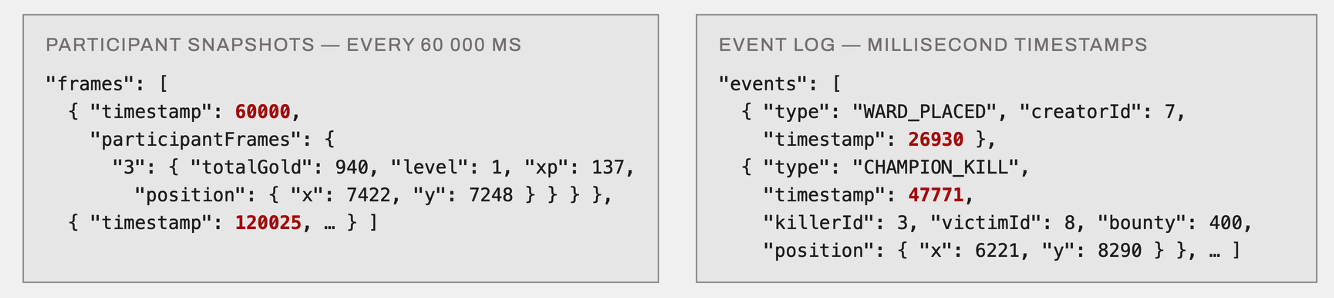
\includegraphics[width=\linewidth]{figures/telemetry_pair.png}
  \caption{참가자 프레임(왼쪽)과 사건 기록(오른쪽)의 예}
  \label{fig:telemetry-pair}
\end{figure}


이 구조가 본 논문의 모든 설계를 규정한다. 챔피언 사이에 오간 피해는 사건으로 기록되지 않는다. 피해와 체력은 1분마다의 프레임에만, 그리고 각 사망에 붙은 요약으로만 나타난다. timeline이 밀리초 단위로 시각을 찍고 지도 위에 위치를 놓는 유일한 챔피언 대 챔피언 전투 사건은 \emph{챔피언 킬}이다. 따라서 관측 가능한 교전 후보의 범위는 적어도 하나의 챔피언 킬을 포함하는 국면으로 제한된다. 본 논문은 킬 사건을 교전 사례를 구성하기 위한 관측 기준으로 사용한다(제 \ref{sec:eng-killless} 절).

``비동기''라는 말은 프레임과 사건 기록의 시간 해상도가 다르고 같은 시각에 맞춰져 있지 않다는 뜻이다. 그림의 챔피언 킬은 47\,771에 있는데, 왼쪽에 그려진 프레임은 60\,000과 120\,025이다. 킬이 그 프레임보다 이르므로, 60\,000의 골드와 위치는 그 킬 시각의 상태가 아니다. 어떤 시각 $t$에서의 상태는 $t$ 이전의 마지막 프레임과 $t$까지의 사건을 합쳐 재구성할 수밖에 없다. 프레임의 나이, 곧 마지막 프레임 이후 흐른 시간은 그 상태 관측이 얼마나 오래되었는지를 나타낸다. 본 논문은 이 재구성을 명시적 시간 계약으로 고정한다(제 \ref{sec:data-contract} 절).
